\documentclass{article}

\usepackage[utf8]{inputenc}

% Figures
\usepackage{graphicx}
\usepackage{float}

% Tables
\usepackage{makecell}
\usepackage{multirow}
\usepackage{rotating}
\usepackage{booktabs}

% BibTeX configuration
\usepackage{biblatex}
\bibliography{references} 
\RequirePackage{doi}
\usepackage{hyperref}




\title{Paths in the labyrinth}
\author{Yannick Lang\\
    \small yannick-stephan.lang@stud.uni-bamberg.de}

\date{ \vspace{0.5cm} \large 
  SME-PHY-B\\ 
  \emph{Physical Computing} \\ \vspace{0.2cm}
  Otto-Friedrich-Universität Bamberg \\ \vspace{0.2cm}
  Summer Term 2022}



\begin{document}

% Custom Commands
\newcommand{\IIC}{I\textsuperscript{2}C}

\maketitle

% Main contents
\section{Introduction}
The following paper describes an arduino based system capable of distinguishing types of junctions via ultrasound.

The problem has been touched upon in \cite{article}. For this project, the focus lies on classification of the environment into corridor, X-Junction or T-Junction. Classification is performed after capturing distance measurements during a $180\deg$ turn of the arduino platform from left to right.

Quick note about Terminology: Unlike \cite{article}, angles will be used from $0\deg$ for the left path, up to $180\deg$ for the right path.
\section{Setup}
\label{sec:setup}

The following section describes the physical components for the project, 
starting with the actual hardware and also covering the environment.
\subsection{Hardware}
\label{subsec:hardware}

From a hardware perspective, two main platforms are used: an arduino micro controller which captures the output from the sensors and a laptop, which processes the data.

\paragraph{Arduino}
This consists of an arduino Nano v.3, a MPU6050 used for its gyroscope sensor and an ultrasonic sensor (HCSR04). The wiring can be seen in Figure \ref{fig:schematic}.

\begin{figure}
    \centering
    \includegraphics[width=0.5\linewidth]{figures/schematic_bb.pdf}
    \caption{Wiring of the Sensors.
        Both sensors are mounted upright, with the ultrasonic sensor aimed at the top of the image. Note: this may cause the order of pins to be reversed, wiring in the schematic is according to the labels, not the order.}

    \label{fig:schematic}
\end{figure}


\paragraph{Laptop}
The arduino is connected via mini USB cable to a laptop, which provides the micro controller with power and receives and evaluates sensor data from it.
To enable a smooth rotation, a angled USB cable may be used, but this is not necessary.
While the receiver does not need to be a Laptop, for instance a Desktop computer or even a raspberry pi could be used instead, I will refer to this component as a Laptop in the following sections.
\subsection{Environment}
\label{subsec:environment}

For this project, the breadboard, on which the arduino and both sensors are connected, is mounted on a swivel plate.
This allows the for easy and smooth rotation.
The board should be mounted in a way that puts the ultrasound sensor close to its center of rotation.

To create the types of junctions that have to be classified, I created two L shaped pieces, consisting of two planks of wood each, joined in a $90\deg$ angle.
Those two are sufficient to create every relevant type of environment.

% TODO: include pictures of expected data and setup
\section{Software}
\label{sec:software}

The software for this project consists of two main parts: 
The code for the micro controller, written in C, and the code for the laptop, written in Typescript.
This section details the methods used for this project.
\subsection{Arduino}
\label{subsec:arduino}

As stated previously, the code that controls the arduino is written in C.
Its purpose is to configure the sensors, monitor them for new data and relay that to the Laptop when available.
Communication with the MPU6050 sensor happens via the Inter-Integrated Circuit (\IIC) protocol.
Communication with the laptop uses a serial connection via USB at a BAUD rate of 250000.


The main control logic for the micro controller is quite simple. Upon startup, all ports and sensors are configured.
Then, a infinite loop is started, which relays sensor data to the laptop if a new value is available.
Availability of new sensor data is determined via interrupts.

For the MPU6050, a interrupt signals that new data is available. In the interrupt handling routine, a variable is the set to one.
In the main loop, this variable is checked, and if it is one, the x value of the gyroscope is read from the mPU via \IIC.
After sending the data to the laptop via the serial interface, the variable is then reset to 0.

For the Ultrasonic sensor, interrupts are used to determine logic level changes on the pin that is connected to the echo signal of the sensor.
Upon activating the sensor, the interrupt is first fired when the echo signal goes high.
Once that happens, the current value of the 16 Bit counter, which is enabled and set to the 8 times prescaler, is saved.
The next time the interrupt is triggered will be when the echo signal goes back down.
When this happens, the timer value is saved again and another variable is set to one. Analogous to reading the MPU,
this variable is used inside the main loop to determine the availability of sensor data. If this variable is set,
the difference of times, i.e. the duration the echo pin has been high, can be sent to the laptop.

To simplify evaluation at the laptop side, values are sent with a prefix indicating the type of sensor,
followed by a colon, a space, the value to be transmitted and a line break sequence.

\subsection{Laptop}
\label{subsec:laptop}

The reasons I choose Typescript for the Laptop-side software are that this is the language I have the most experience with and that, when used in the context of a webapp, it facilitates easy visualization of data.
This is especially helpful for debugging, but comes at the price of performance, which I assume is lower than what can be achieved with other languages such as C.

\paragraph{Proxy}
Because a webapp cannot directly access the serial port, I wrote a proxy script, which reads from the serial port and provides received data via the WebSocket protocol.

\paragraph{Detecting a Rotation}
Detection of a $180\deg$ rotation from left to right is implemented via a state machine.
The relevant sensor values for this detection is the X value of the gyroscope on the MPU6050.
Because the values are not 0 even when the board is completely still, I decided to use the first 50 received values for calibration.
This means that the board should be stable for the first about 2 seconds (see chapter \ref{sec:benchmark}) after connection with the laptop is established.
Those values are used to calculate mean and standard deviation.

If a received value is then within $x$ times the standard deviation of the mean, the platform is considered to not be turning.
If the value is above or below the threshold, the state machine goes to the Over/Under states respectively.
Because outliers are still possible, there are further states, namely Over_Steady and Under_Steady. 
While in the Over/Under states, a counter is maintained, which is increased for each measurement outside the threshold and decreased if the platform is stable again.
If the counter reaches 0, the state returns to the standard, i.e. Steady. If the counter reaches a threshold, the state changes to Over_Steady or Under_Steady depending on previous state.
While these additional states are not currently utilized, they allow to further customize the detection behavior.

While in the Over or Over_Steady states, if value significantly under mean is detected, state is instantly reverted back to Steady and the current rotation ends.

Start of rotation is therefore detected when the state changes away from Steady and end of rotation upon returning to Steady.
For detecting the length of rotation, the sensor values are summed up while state is not Steady.
After a rotation ends, this value can be compared against thresholds to determine what direction this turn was (corresponds to the sign of the sum) and how big the turn was (corresponds to the absolute value of the sum).

% TODO: include visualization of state machine 

\paragraph{Capturing Ultrasound Data}

\paragraph{Normalizing Data}
Due in part to the variable update rate, which is discussed in Section \ref{subsec:benchmark}, the captured readings need to be normalized.
This is done by using the sum of gyroscope readings starting from the beginning of rotation as x-coordinate for the current distance reading.
The total sum of gyroscope readings for a rotation then corresponds to $180\deg$ and other values can be scaled accordingly.
While the gyroscope readings give a speed of rotation rather than a distance, a Sum should still work given the very steady frequency of updates from the MPU (see chapter \ref{benchmark}).
For distance of rotation would be speed of rotation multiplied by time, if we have constant time a simple sum should suffice.
Distances are also scaled to a range between 0 and 1 for the shortest and longest measured distance respectively.

% TODO: describe problem with graphing environment

\paragraph{Evaluating Data}
\section{Analysis}
\label{sec:analysis}
\subsection{Benchmarks}
\label{subsec:benchmark}

\paragraph{Frequency of Updates}
To determine the frequency of updates, values received per second where averaged over 100 seconds.
The rate of updates from the gyroscope is very steady, at between 31 and 32 Updates per second.
The frequency of new values from the ultrasound sensor is not as steady, as it depends on the distance being measured.
This is because longer distances take longer to measure, and the arduino immediately starts a new measurement upon completion.
In general, distance measured and update frequency are inversely proportional, i.e. with longer distance the rate of updates decreases.
At 10cm distance, update frequency is about 75Hz, and decreases roughly by about 10hz per meter, see \ref{fig:benchmark}.

\begin{table}
    \centering
    \begin{tabular}{l|lll}
            & Gyroscope & Ultrasound & \\
        \cline{1-3}
        10  & 31.48979  & 74.9898    & \\
        20  & 31.48979  & 73.77319   & \\
        30  & 31.55670  & 72.02040   & \\
        50  & 31.57731  & 73.82653   & \\
        75  & 31.62886  & 72.11224   & \\
        100 & 31.60821  & 65.42857   & \\
        150 & 31.50515  & 55.66326   & \\
        200 & 31.62244  & 53.83673   &
    \end{tabular}

    \caption{Distance in cm from sensor and update frequency}
    \label{table:benchmark}
\end{table}

\begin{figure}
    \centering
    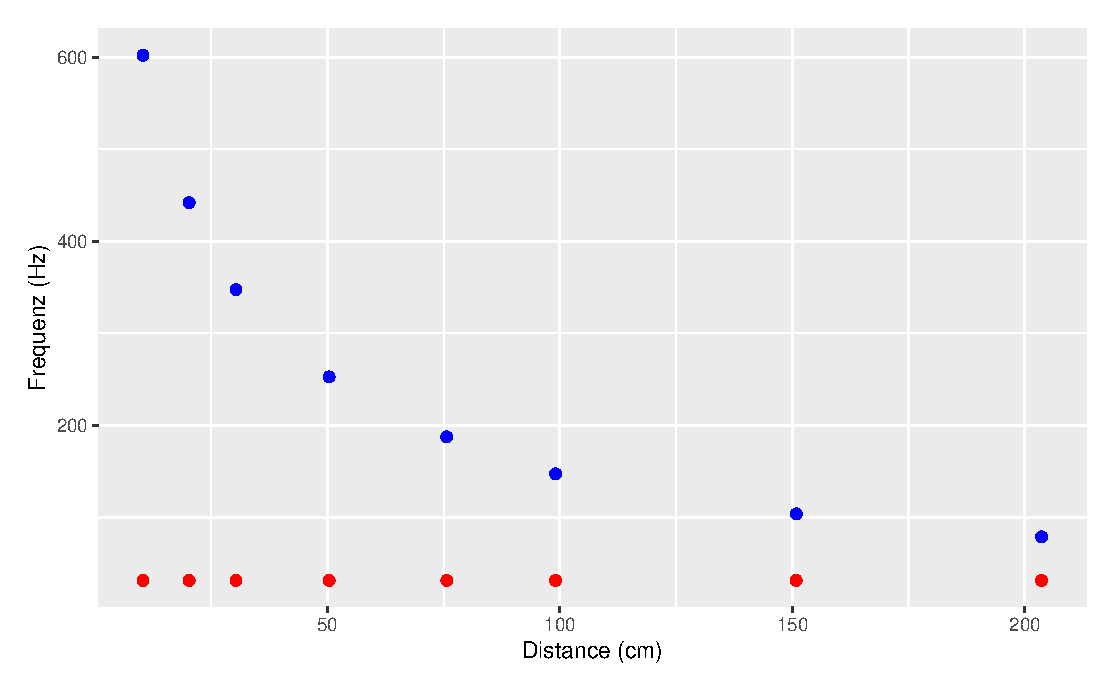
\includegraphics[width=0.5\linewidth]{figures/benchmark.eps}
    \caption{The data from \ref{table:benchmark} visualized}
    \label{fig:benchmark}
\end{figure}


\subsection{Known Problems}

The following sections discusses some of the problems I faced, and solutions or mitigations I employed.

\paragraph{Incorrect Ultrasonic Measurements during \IIC communication}
During an earlier stage of the project, Ultrasonic measurement received immediately after Gyroscope reading were off
by a lot.
While this does not seem to be an issue anymore, I am neither sure what caused this nor why it works now.
Potential mitigation strategies for this would have been laptop sided, were values received right after gyroscope data
could either be dropped or substituted by a suitable average.


\paragraph{Unknown path width}
Classification could be much simpler if path width was known. Three distance measurements would suffice for classification, one at 0, one at 90 and one at 180 Degrees.
A X Junction would have all three measurements larger than path width,
T Junction would have first and third measurement larger, second measurement equal to path width (technically more like half path width) and
a corridor would just have the second measurement greater than path width.
My first idea was to use the distance measurements at $45\deg$ and $135\deg$, where the corners would be expected for a X Junction, to estimate this variable.
This did not turn out to be a workable approach for several reasons.
First, the ultrasonic sensor fails to get reliable readings for the distance if the object is at too much of an angle.
Secondly, this approach would only be useful for X-Junctions, as the other two types do not have the corners necessary.

This did not turn out to be a problem after all, since classification now works based on similarity to past data and should due to normalization be somewhat independent of path width.

\paragraph{Graphing the environment from the scan data} Probably as a result of the difficulty to get measurements at an angle, the data cannot be easily graphed to show the scanned environment.
Considering our data consists of angles and distances, it can be understood as polar coordinates.
Therefore, converting it to cartesian coordinates and plotting those should give a pretty good image of the junction.
This works very well in theory, but not as well with values actually measured by the sensors, see Figure \ref{fig:cartesian}.
This is not of much importance to the overall project, but would have been helpful for visualization.

\begin{figure}[H]
    \centering
    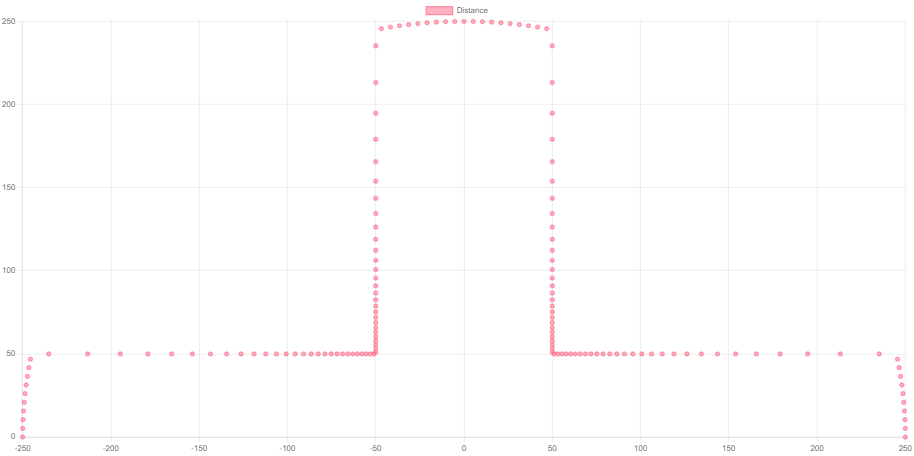
\includegraphics[width=0.45\linewidth]{figures/cartesian_simulated.png}
    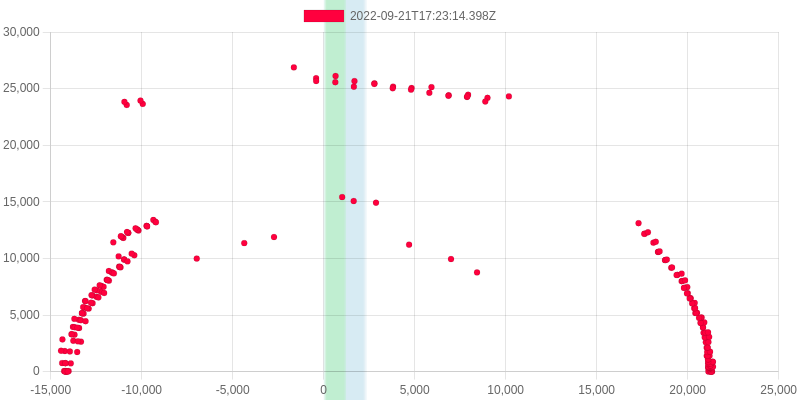
\includegraphics[width=0.45\linewidth]{figures/cartesian_actual.png}
    \caption{Left: simulated data, converted to cartesian coordinates and
        graphed.
        Right: actual data, converted to cartesian coordinates and graphed.
        Notice the missing sections, that are mostly obstacles at an angle.}

    \label{fig:cartesian}
\end{figure}

\paragraph{Turns are not detected correctly} When a turn ends, the calculated angle is logged to the console. If this is off, the most likely reason for this that the platform was not stable during calibration. To fix this, simply reload the app and make sure the platform does not turn for one or two seconds, until the calibration is done.

\section{Summary}
\label{sec:summary}

This paper describes the process of building a platform for distinguishing x junctions, t junctions and corridors via a gyroscope and a ultrasonic distance sensor.
Turns of the platform are reliably detected via a state machine.
Upon detection, data that has been recorded during the rotation is used to compare the scan of the environment against previously recorded data, thus allowing a classification.

% Please clean your references! 
% See https://sites.umiacs.umd.edu/elm/2018/12/13/the-art-of-clean-references/
\printbibliography

\end{document}